% =========================================================================== %
\chapter{Описание реализованных средств}\label{chap4_soft_testing}
% =========================================================================== %
% --------------------------------------------------------------------------- %
\section{Использованные технологии}\label{sec:used_tech}
% --------------------------------------------------------------------------- %
В процессе разработки компонентов новой версии программного каркаса comsdk были использованы некоторые его ранее созданные компоненты. Так, среди прочих, был использован класс для представления данных в виде универсального ассоциативного массива \textsf{Anymap}. В данный ассоциативный массив записываются входные данные для алгоритма из файла формата .aINI\cite{SokAINI}. Данный класс позволяет хранить разнотипные данные в одном объекте с использованием строковых ключей для доступа к ним. Кроме того, в данном классе реализована возможность экспорта данных в файл в формате aINI.

Кроме того, был использован уже реализованный инструментарий для загрузки функций из скомпилированных динамических библиотек и интерфейс функциональной возможности \textsf{ActionItem}.

Реализация проводилась с использованием стандарта языка C++ C++-11 и стандартной библиотеки шаблонов (англ.~Standard Template Library (STL)).

% --------------------------------------------------------------------------- %
\section{Алгоритмы}\label{sec:algorithm_desc}
% --------------------------------------------------------------------------- %
Для определения общей логики обхода графовой модели без учёта возможности обхода параллельных ветвей был разработан упрощённый алгоритм, поддерживающий только условное ветвление. Его блок-схема представлена на рисунке~\ref{fig:flowchartNoBranching}.
\begin{figure}[H]
    \centering
    \includegraphics[height=0.6\textheight]{figures/flowchart.graphRunning1.png}
    \caption{Блок-схема алгоритма обхода графовой модели, не предполагающей параллельное исполнение}
    \label{fig:flowchartNoBranching}
\end{figure}

Был отдельно рассмотрен случай, когда необходимо параллельно обойти несколько ветвей. Для контроля за параллельным исполнением функций перехода и выполнения необходимых операций по распределению и сбору данных с задействованных вычислительных ресурсов была разработана управляющая струкутура ``контейнер выполнения''. Более подробно она описана в разделе~\ref{chap3_soft_architecture}. Логика работы с данной структурой представлена на рисунке~\ref{fig:flowchartExecutionContainer}.
\begin{figure}[!ht]
    \centering
    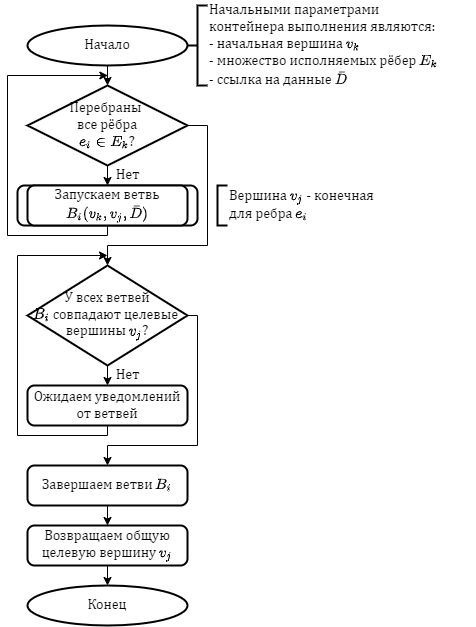
\includegraphics[height=0.45\textheight]{figures/flowchart.executionContainer.png}
    \caption{Блок-схема алгоритма отслеживания параллельного исполнения ветвей графа}
    \label{fig:flowchartExecutionContainer}
\end{figure}

При этом в процессе работы метода \textsf{run()} управляющей структуры ``контейнер выполнения'' подразумевается создание отдельных ``ветвей''.

Алгоритм обхода одной ветви представлен на рисунке~\ref{fig:flowchartExecutionBranch}.

\begin{figure}[!ht]
    \centering
    \includegraphics[width=0.8\textwidth]{figures/flowchart.executionBranch.png}
    \caption{Блок-схема алгоритма исполнения одной из параллельных ветвей}
    \label{fig:flowchartExecutionBranch}
\end{figure}

Общий алгоритм предполагает завершение выполнения ветви по сигналу от ``контейнера выполнения''. Ситуация, когда по какой-то причине для текущей вершины $v_i$ и данных $\bar{D}$ не было выбрано ни одного ребра, является исключительной и должна обрабатываться отдельно.

Разработанная логика параллельного обхода ветвей графа была добавлена к исходному алгоритму. Итоговая блок-схема разработанного алгоритма обхода представлена на рисунке~\ref{fig:flowchartFinal}.

\begin{figure}[!ht]
    \centering
    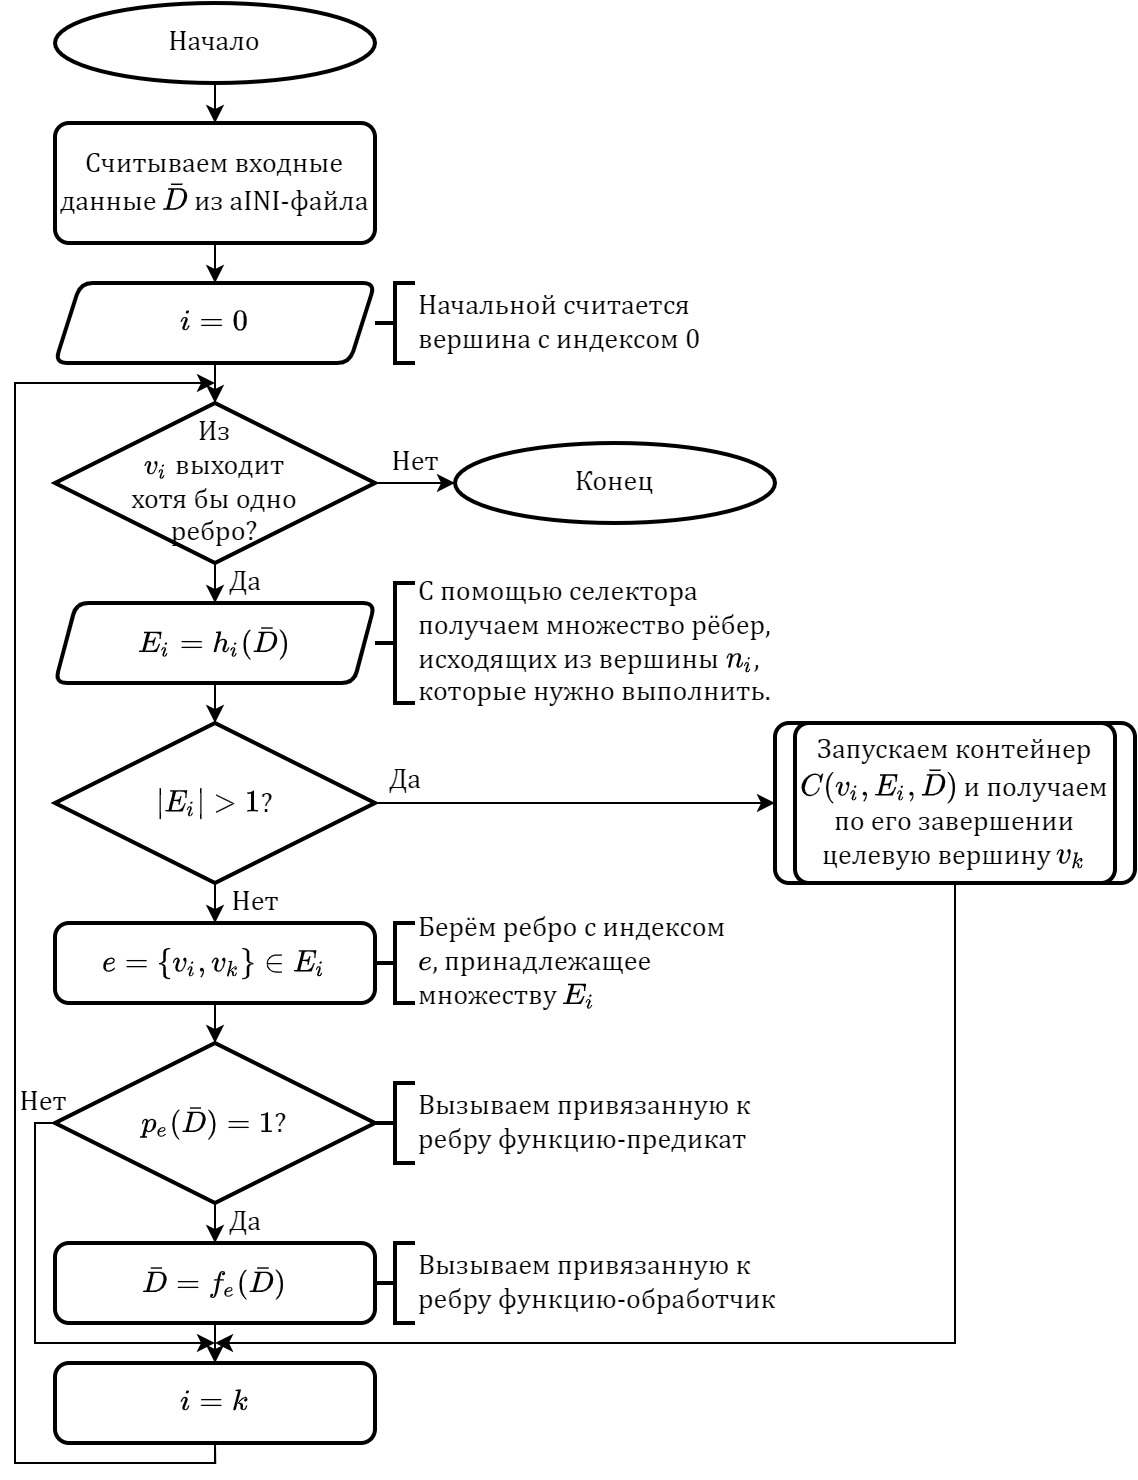
\includegraphics[height=0.6\textheight]{figures/flowchart.graphRunning2.png}
    \caption{Блок-схема алгоритма обхода графовой модели}
    \label{fig:flowchartFinal}
\end{figure}

Таким образом, дальнейшие реализации конкретных вариантов параллельного обхода ветвей с задействованием различных вычислительных ресурсов (потоков процессора, процессов, узлов кластера и~т.д.) должны будут создаваться в соответствии с разработанным алгоритмом.

% --------------------------------------------------------------------------- %
\section{Сборка и тестирование}
% --------------------------------------------------------------------------- %
Для сборки разработанных программных средств требуется библиотека Boost, компилятор языка С++, поддерживающий стандарт C++-11, и система сборки CMake. При разработке и отладке использовался компилятор gcc и библиотека Boost версии 1.78.

Для реализованных компонентов были разработаны unit-тесты для проверки корректности их внутренней логики. Разработанные юнит-тесты были размещены в директории comsdk/test (см. рисунок~\ref{fig:fileStructure}). В частности, для тестирования возможности загрузки функций-предикатов и обработчиков из динамических библиотек была создана динамическая библиотека с простыми тестовыми функциями.


Для тестирования разработанных средств необходимо в корневой папке проекта создать директорию build, перейти в неё и выполнить в ней следующую последовательность команд:

\texttt{cmake -DCMAKE_BUILD_TYPE=Release ..}

\texttt{make -j4},

где флаг \textsf{DCMAKE_BUILD_TYPE} отвечает за тип сборки проекта. Возможные типы:
\begin{itemize}
    \item Debug -- файлы библиотеки comsdk, библиотеки для тестов и бинарные файлы тестов будут размещены в директории build-debug;
    \item Release -- файлы библиотеки comsdk, библиотеки для тестов и бинарные файлы тестов будут размещены в директории build-release.
\end{itemize}

После этого необходимо запустить утилиту CTest, которая использовалась для прогона юнит-тестов.